        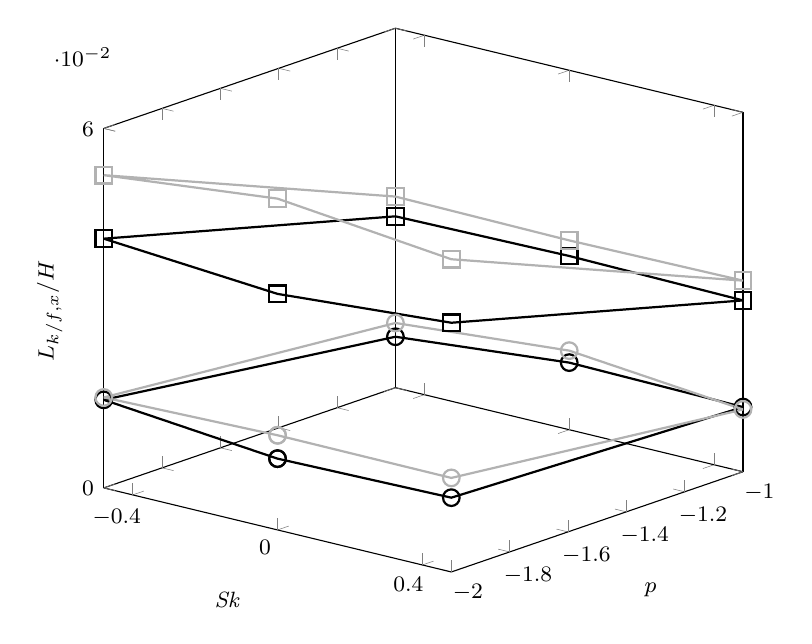
\begin{tikzpicture}[]
        \centering
        \begin{axis}[
        view={40}{20},
            ylabel={$p$},
            xlabel={\textit{Sk}},
			zlabel={$L_{k/f,x}/H$},
			xtick={-0.4,0,0.4},
			ztick={0,0.06},
			zmin=0,zmax=0.06,
            %ymin=0, ymax=0.16,
            width=.8\textwidth,
            height=.7\textwidth,
            label style={font=\footnotesize},
            tick label style={font=\footnotesize}
            ]
            
            
            
                                    \addplot3 [
            black,mark=o,thick, mark size=3pt
            ]
            coordinates{
            (0,-2,0.0119)			
			(0.48,-2,0.0124)
			(0.48,-1,0.0108)
			(0,-1,0.0112)
			(-0.48,-1,0.0085)
			(-0.48,-2,0.0147)
            (0,-2,0.0119)
			};
			\addplot3 [
            gray!60,mark=o,thick, mark size=3pt
            ]
            coordinates{
            (0,-2,0.0158)
			(0.48,-2,0.0157)
			(0.48,-1,0.0104)
			(0,-1,0.0132)
			(-0.48,-1,0.0108)
			(-0.48,-2,0.0151)
			(0,-2,0.0158)
            };
            
            
        
            
                                    \addplot3 [
            black,mark=square,thick, mark size=3pt
            ]
            coordinates{
            (0,-2,0.0394)			
			(0.48,-2,0.0416)
			(0.48,-1,0.0286)
			(0,-1,0.0290)
			(-0.48,-1,0.0286)
			(-0.48,-2,0.0416)
            (0,-2,0.0394)
			};
			\addplot3 [
            gray!60,mark=square,thick, mark size=3pt
            ]
            coordinates{
            
            (0,-2,0.0553)
			(0.48,-2,0.0522)
			(0.48,-1,0.0319)
			(0,-1,0.0316)
			(-0.48,-1,0.0319)
			(-0.48,-2,0.0522)
			(0,-2,0.0553)
            };
            
        \end{axis}
        \end{tikzpicture}